\section{Implementation}
In this section, we will describe the implementation of bisection and twisted algorithm on GPU.
GPU chooses Single Program Multiple Threads (SPMT) mode for its scheduling. 
A thread is the fundamental working unit of a parallel program.
A warp with continuous 32 threads works concurrently.
A block is a group of multiple threads sharing the shared memory.
Based on the algorithm and the GPU architecture, the implementation can be separated into two steps one after another.
The first one is singular value kernels and the last one is singular vector kernels.
In the end of this section, we also introduce an implementation when matrix size becomes huge.

\subsection{Singular Value Kernels}
In the singular value design, we have two steps to obtain the singular values.
\begin{enumerate}
\item Seperate the whole interval into several subintervals in parallel.
\item Obtain the singular values in these subintervals in parallel.
\end{enumerate}

\begin{figure}[hbpt]
\centering
  \subfigure[Equal Length Division]
  {
  \includegraphics[width=0.5\textwidth]{length_interval}
  \label{fig:length_interval}
  }
  \subfigure[Equal Number Division]
  {
  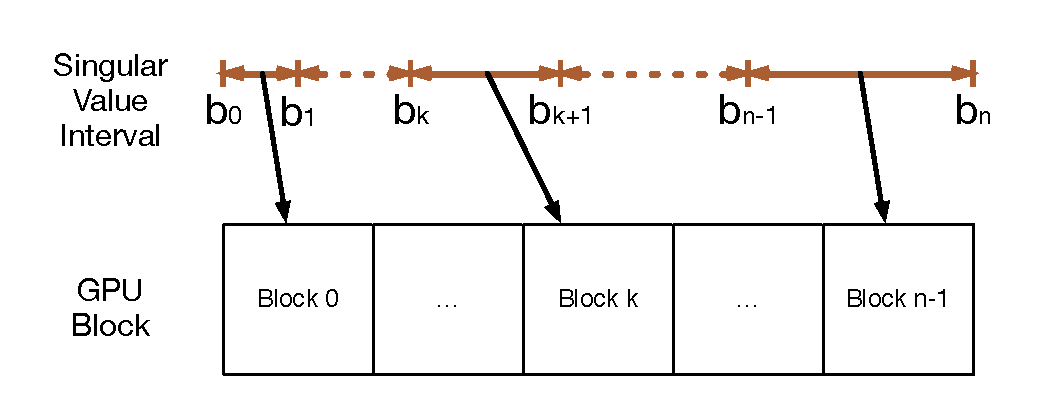
\includegraphics[width=0.5\textwidth]{number_interval}
  \label{fig:number_interval}
  }
  \caption{Division Strategies of interval}
\end{figure}
For the first step, we design the strategy to separate the interval by the length shown in Fig.\ref{fig:length_interval}.
In this strategy, we divide the whole interval $[a_0, a_n)$ into $n$ subintervals with the same length, while every subinterval may not have the same number of singular values usually.
In mathematical word, this strategy can be expressed as% $a_{k+1}-a_k = a_{k}-a_{k-1}$ and $NegCount(b_{k+1})-NegCount(b_{k}) \ne NegCount(b_{k})-NegCount(b_{k-1})$.
\begin{eqnarray}
a_{k+1}-a_k = a_{k}-a_{k-1} \hspace{2cm} \\
NegCount(a_{k+1})-NegCount(a_{k}) \ne \hspace{1cm} \nonumber\\
NegCount(a_{k})-NegCount(a_{k-1})
\end{eqnarray}

\begin{algorithm}
%\small
\caption{Equal Length Subinterval Algorithm}
\label{alg:lengthsub}
\begin{algorithmic}[1]
\Procedure{$\mathbf{Length\_Divide}$}{$n, B, t, \tau$}
  \State Obtain singular value boundary $[l,u)$ of matrix $B$;
  \State Define the thread ID $i$, $i<t$;
  \State Obtain average step $s = (u-l) / t $;
  \State Lower bound $\alpha = l + i * s$;
%  \State Upper bound $\beta = max(l + (i+1) * s, \alpha)$;
  \State $n_{\alpha} = NegCount(\alpha)$;
%  \State $n_{\beta} = NegCount(\beta)$;
%  \State $\alpha = \min(\alpha,\beta)$;
%  \State $\beta = \max(\alpha, \beta)$;
%  \State $n_{\alpha} = \min(n_{\alpha},n_{\beta})$;
%  \State $n_{\beta} = \max(n_{\alpha}, n_{\beta})$;
%  \State Max scan to refine $\alpha, \beta, n_{\alpha}, n_{\beta}$
%  \State Call $Bisection(val, n, B, \alpha, \beta, n_{\alpha}, n_{\beta}, \tau)$
  \State save the division point $\alpha$ and $n_{\alpha}$
\EndProcedure
\end{algorithmic}
\end{algorithm}

The parallel algorithm of length division working in GPU threads is shown in Algorithm \ref{alg:lengthsub}.
The length division strategy is easy to design.
However, it is not flexible to determine the number of subintervals for a better speedup.
This is because the determination of number of blocks is based on multiple aspects, such as the maximum number of threads, the number of threads in GPU warp, and the size of matrix.
The maximum number of threads per block determines the minimum number of blocks should be allocated.
The number in threads in GPU warp makes sure the suitable subintervals for best GPU utilization level.

Even we separate the interval with the best GPU utilization level, the speedup of length division cannot also reach a high level.
To achieve a even better speedup, we use another strategy to spearate the whole interval by the number of singular values in Fig.\ref{fig:number_interval}.
In this strategy, we divide the interval $[b_0,b_n)$ into $n$ subintervals with the same number of singular value.
However, the length of the subinterval may not be equal to others.
The mathematical representation can be writed as %$NegCount(b_{k+1})-NegCount(b_{k})=NegCount(b_{k})-NegCount(b_{k-1})$ but $b_{k+1}-b_k \ne b_{k}-b_{k-1}$
\begin{eqnarray}
b_{k+1}-b_k \ne b_{k}-b_{k-1} \hspace{2cm} \\
NegCount(b_{k+1})-NegCount(b_{k}) = \hspace{1cm} \nonumber\\
NegCount(b_{k})-NegCount(b_{k-1})
\end{eqnarray}
The parallel algorithm with same number of singular value is shown in Algorithm \ref{alg:numsub}.
\begin{algorithm}
%\small
\caption{Equal Number of Singular Value Subinterval Algorithm}
\label{alg:numsub}
\begin{algorithmic}[1]
\Procedure{$\mathbf{Number\_Divide}$}{$n, B, t, \tau$}
  \State Obtain singular value boundary $[l,u)$ of matrix $B$;
  \State Define the thread ID $i$, $i<t$;
  \State $mid = inside(l, u, B)$;
  \State $n_m = NegCount(n, B, mid)$;
  \While {$n_m \ne (i+1)n/t$ and $mid-l > \tau$}
    \If {$n_m \ge (i+1)n/t$}
      \State $u=mid$;
      \State $n_u=n_m$;
    \Else
      \State $l=mid$;
      \State $n_l=n_m$;
    \EndIf
    \State $mid = inside(l, u, B)$;
    \State $n_m = NegCount(n, B, mid)$;
  \EndWhile
  \State save the division point $mid$ and $n_m$.
\EndProcedure
\end{algorithmic}
\end{algorithm}


We calculate the boundary points of the subintervals from the first step based on Algorithm \ref{alg:lengthsub} and Algorithm \ref{alg:numsub}. 
Either algorithm works in one block with multiple threads.
Every thread is responsible for one spliting point.
The second step is to calculate the exact singular values in these subintervals with Algorithm \ref{alg:bisection}.

In our design, one subinterval is allocated into one GPU block.
In other words, one GPU block will calculate all the singular values in its corresponding subinterval.
%Suppose the whole interval can be divided into $N$ subintervals, every block processes one subintervals, and thus $N$ blocks are needed.
Inside the block, multiple threads are working concurrently.
One thread will obtain one singular value in the subinterval.
%Suppose the number of singular values in one block is $M$, thus $M$ is the number of threads in the block.

\subsection{Singular Vector Kernel}
The singular vector kernel is designed based on Algorithm \ref{alg:twisted}.
First, we achieve the algorithm without any optimization.
But the 10X speedup compared to CPU is low because of the heavy usage of global memory and the low global memory throughput.
After we utilize the local memory and shared memory instead of frequent-used global memory and change the matrix arrangement from row-major to column-major.
The performance nearly doubled.

\subsection{Huge Size Solution}
When the matrix size becomes more than a certain level determined by GPU memory, the singular vector kernel cannot obtain all the singular vectors at the same time.
In this subsection, we introduce a divide-and-conquer architecture to solve the huge matrix size.

Due to the disivibility of the bisection and twisted algorithm, we can easily separate the whole interval into several subsections.
The GPU calculates one subsection at the same time.
After one subsection is finished, GPU processes the next one, until the last one.
Thus, the execution time is the summation of every subsection.

\textbf{Multiple-GPU version}
When matrix size is huge, the performance 
